\noindent\textbf{Question 1:}

\noindent\emph{AIMA 3.13 Describe a state space in which iterative deepening search performs much worse than depth-first search (for example, \BigO{n^2} vs. \BigO{n}):}

In a state space where each state has one single successor state, and the goal state is  located at a depth $n$, DFS will arrive at the goal in $n$ steps. Iterative deepening search will however, first need to run through the iterative step until the depth of the search is $n$. In the first iteration it will preform 1 step, in the second it will preform 2, ... until finally the $n^{th}$ iteration where it performs $n$ steps exactly as the DFS. In this case Iterative Deepening Search is performing \BigO{n^2} steps, or \BigTheta{n^2/2}. See \referenceFigure{Figure_1}

\begin{figure}[htbp]
  \centering
  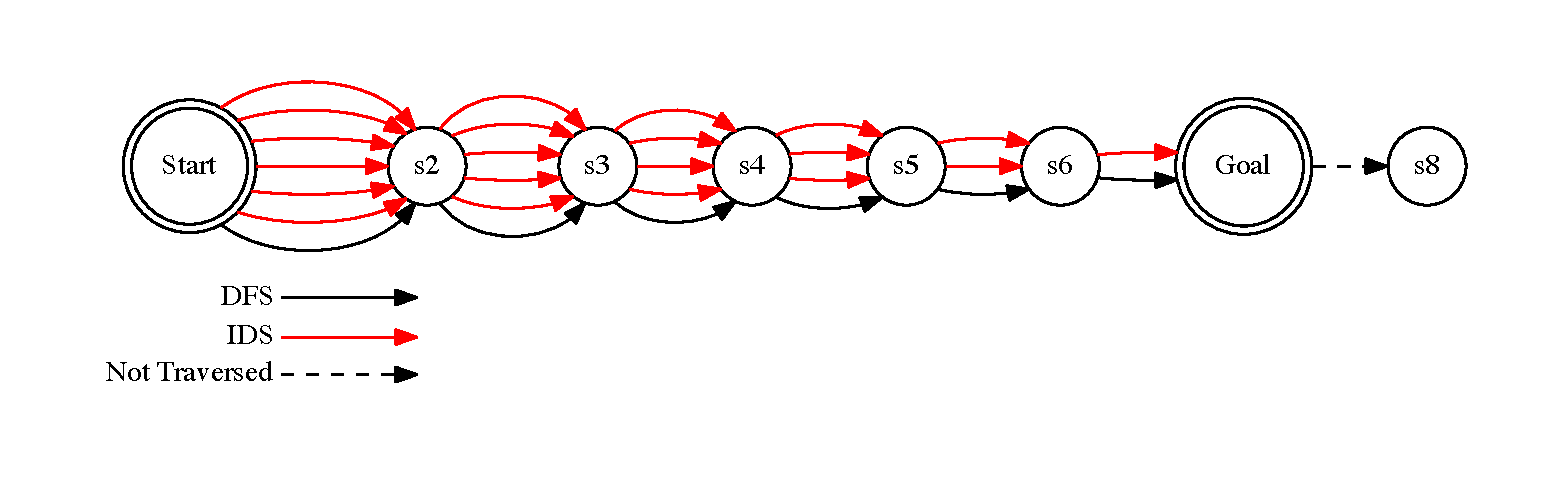
\includegraphics[width=1.0\textwidth]{./media/dfs_vs_ids.pdf}
  \caption{ \label{Figure_1}DFS performs better than IDS in this search space.}
\end{figure}


